\subsection{Aplicação Fábrica: Registo de Produto Acabado}
\subsubsection*{Descrição do caso de uso}
No registo de produto acabado, espera-se que utilizador entre na página e indique o peso do produto acabado. A informação da data deve ser indicada automaticamente pelo sistema. 

\begin{figure}[H] 
	\begin{center}
		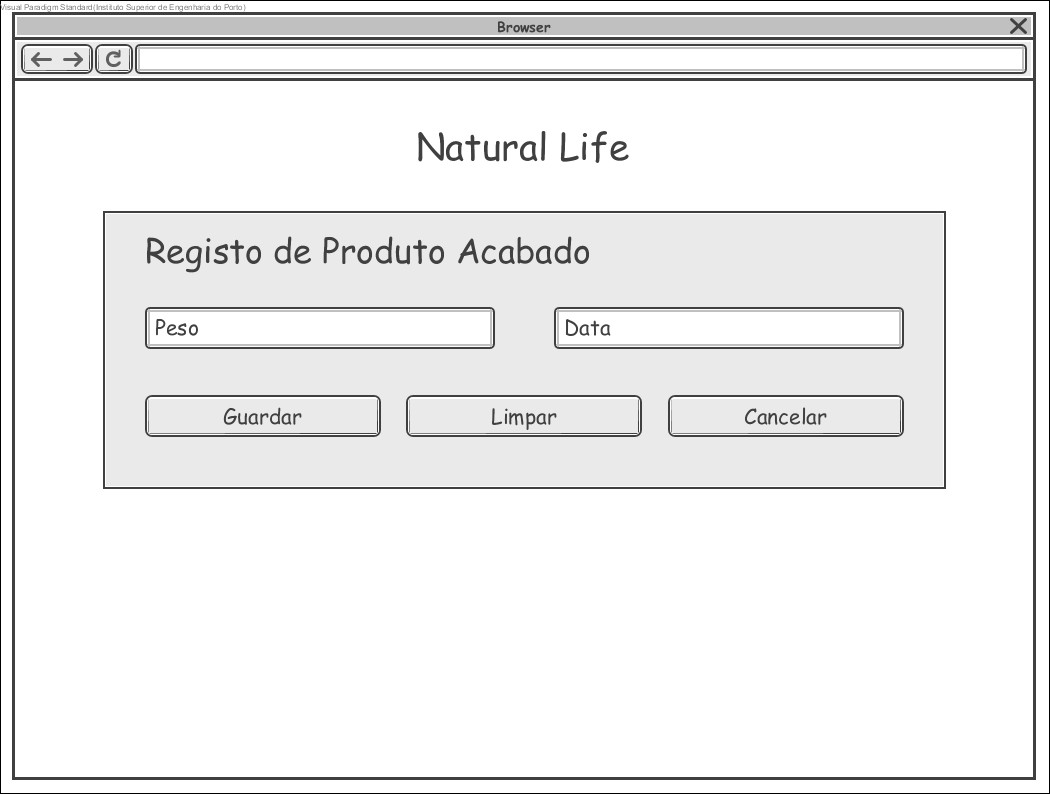
\includegraphics[width=0.60\textwidth,keepaspectratio]{figuras/Diagramas_vp/DI_Fabrica_4_Registo_de_Produto_Acabado.jpg}
		\caption{Modelo do formulário do registo de produto acabado}
		\label{fig:di_prod_acabado} 
	\end{center}
\end{figure}

\subsubsection*{Fluxo do caso de uso}
O caso de uso inicia-se com a abertura da página do registo de produto acabado. É apresentado o formulário com a data previamente preenchida. O utilizador tem de indicar o peso do produto acabado. Após indicar as informações solicitadas precisona o botão "Guardar". No final do registo é apresentada uma mensagem ao utilizador. Caso o registo seja feito com sucesso um novo separador é aberto com o código de barras para ser impresso.


\begin{figure}[H] 
	\begin{center}
		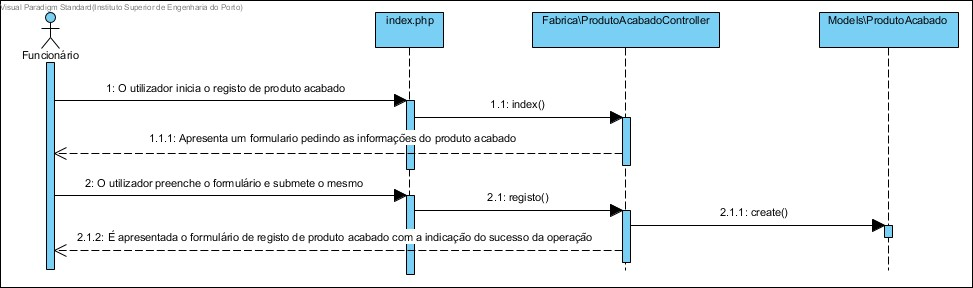
\includegraphics[width=\textwidth,keepaspectratio]{figuras/Diagramas_vp/SD_Fabrica_4_Registo_de_Produto_Acabado.jpg}
		\caption{Diagrama de sequência registo de produto acabado}
		\label{fig:sd_prod_acabado} 
	\end{center}
\end{figure}